\section{Experimental method}
Fig. \ref{fig:t59_detectors} shows a schematic view of the entire set of detectors.
Two central detectors, WAGASCI modules, contain the neutrino target material, water, and plastic scintillator bars,
and are placed along the beam direction.
The muon range detectors (MRDs) consist of two detectors in the side region (side-MRD modules)
and one detector in the downstream region (downstream-MRD) around the central detector.

\begin{figure}%[htbp]
  \begin{center}
  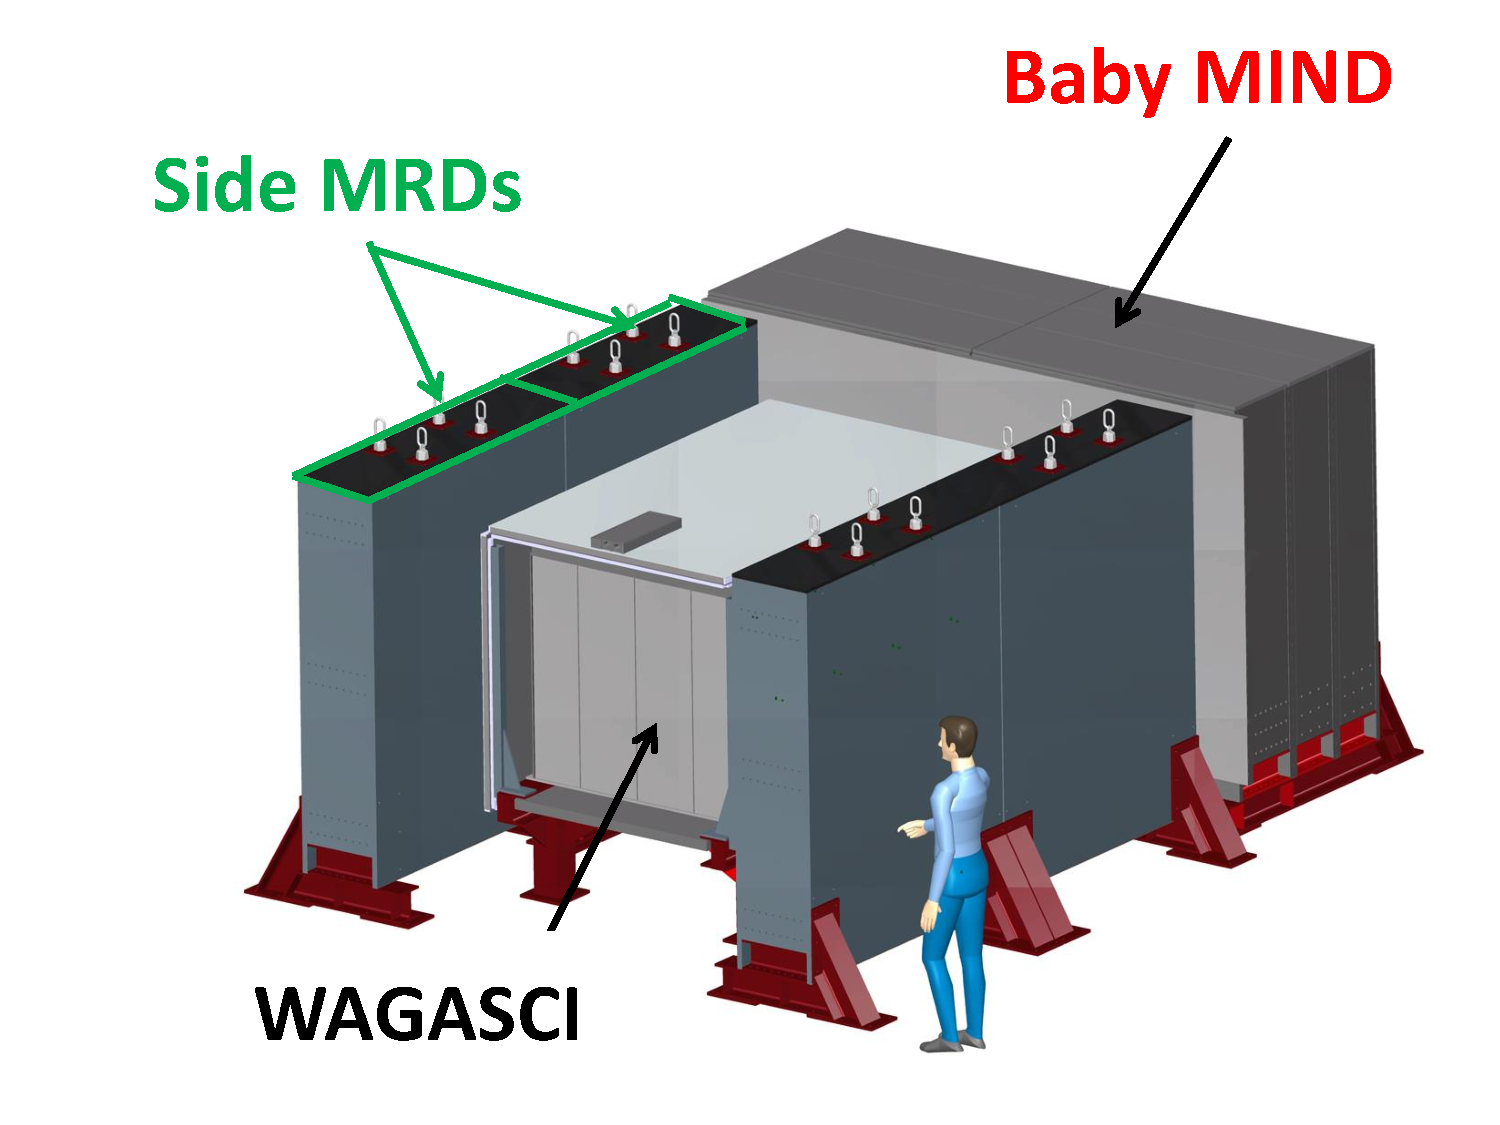
\includegraphics[width=0.6\textwidth]{figs/t59_detectors.pdf}
  \caption{Schematic view of the entire set of detectors.}
  \label{fig:t59_detectors}
  \end{center}
\end{figure}


The dimension of neutrino target region in one WAGASCI module is 
100cm $\times$ 100cm in the x and y directions and 50cm along the beam direction.
The total water mass serving as neutrino target is $\sim$400kg per each module (the remaining $\sim$ 100kg is the plastic scintillator mass).
Inside the WAGASCI modules, plastic scintillator bars are aligned as a 3D grid-like structure,
shown in Fig. \ref{fig:3d_grid_structure}, and spaces in the structure are filled with water.
When neutrinos interact with hydrogen and oxygen in water, charged particles are generated.
Neutrino interactions are identified by detecting tracks of charged particles through plastic scintillator bars.
Thanks to the 3D grid-like structure of the scintillator bars,
the WAGASCI modules have $4\pi$ angular acceptance for charged particles.
Thin plastic scintillator bars (thickness $\sim$ 0.3cm) are used for the WAGASCI modules
to reduce the mass ratio of scintillator bars to neutrino target materials,
because neutrino interactions in the scintillator bars are a background for the cross section measurements.
Scintillator bars whose dimensions are 2.5cm $\times$ 0.3cm $\times$ 100cm are used for the WAGASCI modules.
The total number of channels in the two WAGASCI modules is 1280.

\begin{figure}%[htbp]
  \begin{center}
  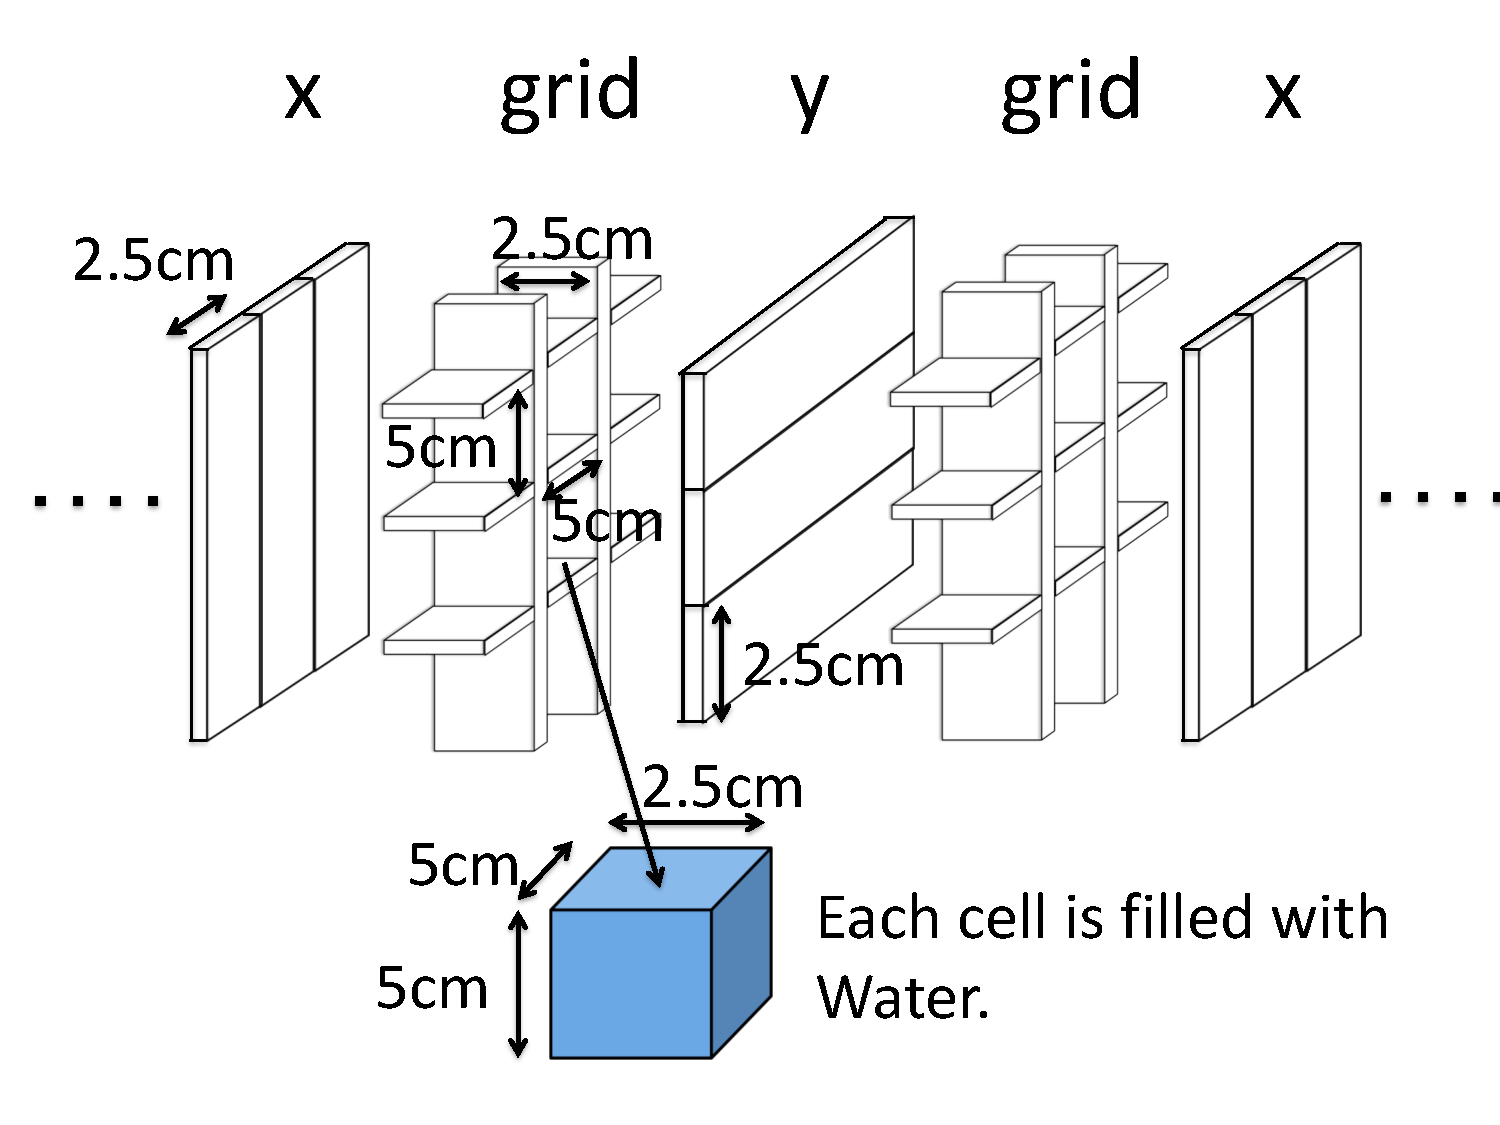
\includegraphics[width=0.6\textwidth]{figs/3d_grid_structure.pdf}
  \caption{Schematic view of 3D grid-like structure of plastic scintillator bars inside the WAGASCI module.}
  \label{fig:3d_grid_structure}
  \end{center}
\end{figure}



The dimension of one side-MRD module is 161cm(width) $\times$ 180cm(height) 
in a plane along the beam direction and 46cm perpendicular to the beam direction.
The module consists of 11 3cm thick iron plates and 10 tracking scintillator planes.
Each tracking scintillator layer of the module has 8 scintillator bars whose dimensions are
20cm(width) $\times$ 0.7cm(thickness) $\times$ 180cm(length) making a plane measuring $160\times180$cm$^{2}$
in the horizontal and vertical directions.
The total number of channels in two side-MRD modules is 160.
The mechanical drawings of the side MRD are shown in Fig. \ref{fig:mec_drawing_side_mrd}.
The total weight of one side-MRD module is less than 10 ton, and it can be moved to the B2 floor using the crane in the NM pit.
The role of the side-MRD modules is the selection of muon tracks from the charged-current (CC) interactions and the rejection of short tracks caused by neutral particles, neutron and gammas,
that originate mainly from neutrino interactions in material surrounding the WAGASCI modules,
like the wall of the detector hall, or neutral-current (NC) interactions.
The muon momentum can be reconstructed from its range inside the module.
The side-MRD modules are located 50cm away from the WAGASCI modules to identify the 
direction of motion of charged particles from the hit-time difference between the two detectors,
and reject charged-particle background that originates from neutrino interactions
in the material surrounding the WAGASCI modules, like the hall of the detector hall and the side-MRD modules themselves.

\begin{figure}%[htbp]
  \begin{center}
  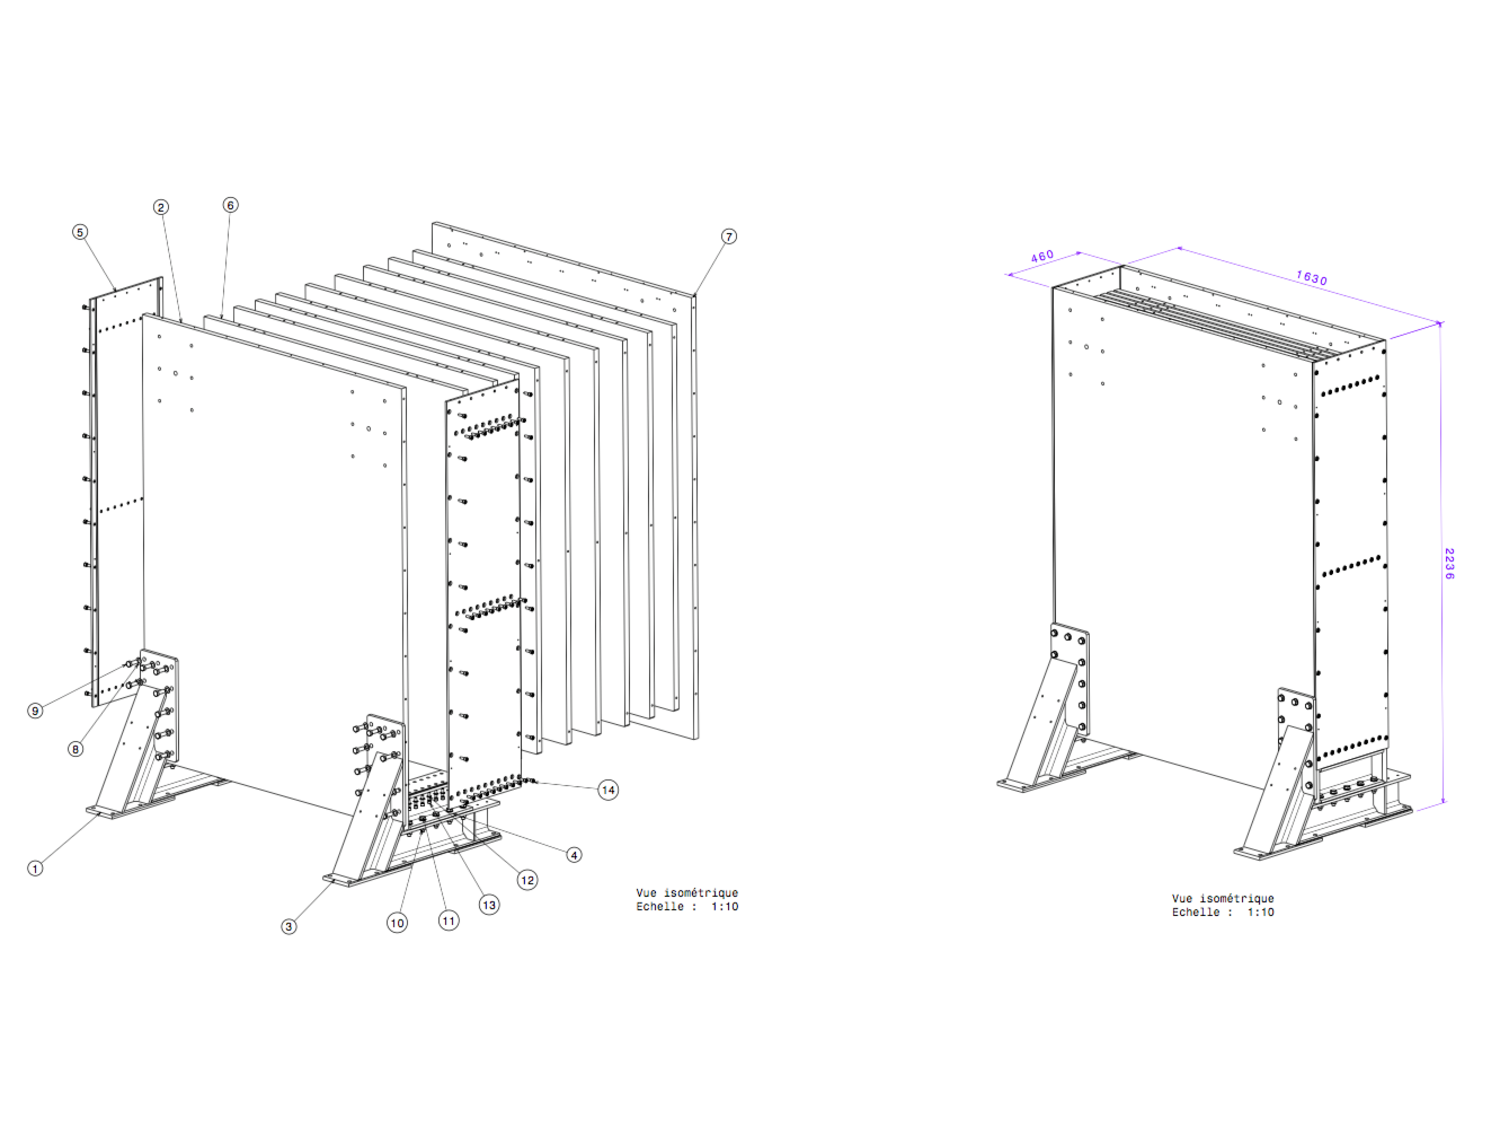
\includegraphics[width=0.8\textwidth]{figs/mec_drawing_side_mrd.pdf}
  \caption{Mechanical drawings of the side-MRD module.}
  \label{fig:med_drawing_side_mrd}
  \end{center}
\end{figure}


As for the downstream-MRD, there is an update from the original proposal.
We have decided to magnetize the downstream MRD to realize high charge identification efficiencies for $\mu^{+}$/$\mu^{-}$ down to 500 MeV/c,
and the Baby MIND\cite{BabyMIND} is used as the downstream-MRD.
The Baby MIND experiment is the approved project by the CERN Research Board in December 2015,
and the Baby MIND is the magnetized MRD developed in the experiment.
The dimension of Baby MIND is XXXcm $\times$ YYYcm 
in a plane perpendicular to the beam direction and ZZcm along the beam direction.
The module consists of N Xcm thick magnetized iron plates and N2 tracking scintillator planes.
Each tracking scintillator layer of Baby MIND has N scintillator bars whose dimensions are
Xcm $\times$ Zcm $\times$ Ycm making a plane measuring $X \times Y$cm$^{2}$
in the horizontal and vertical directions as shown in Fig. \ref{ref:fig:scinti_layer_babymind}.
The total number of channels in the Baby-MIND is N.

\begin{figure}%[htbp]
  \begin{center}
  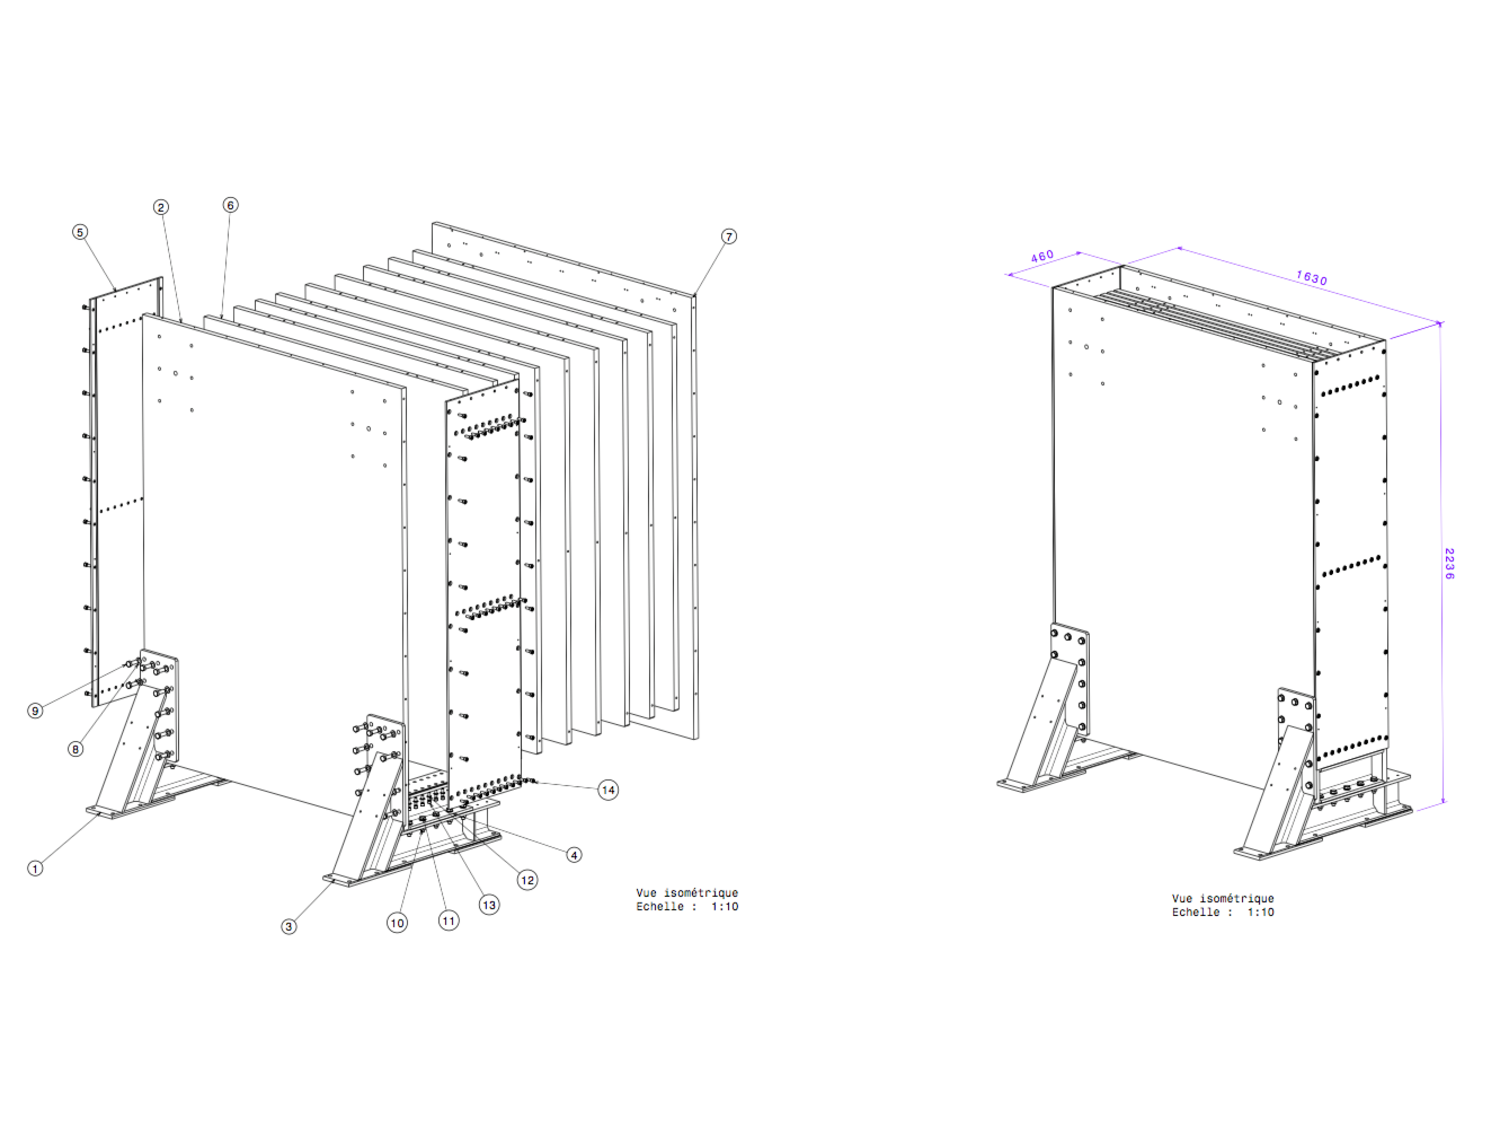
\includegraphics[width=0.8\textwidth]{figs/mec_drawing_side_mrd.pdf}
  \caption{Mechanical drawings of the side-MRD module.}
  \label{fig:med_drawing_side_mrd}
  \end{center}
\end{figure}


Scintillation light in the scintillator bar of WAGASCI modules and MRDs is collected and transported to a photodetector with a wavelength shifting fiber (WLS fiber).
The light is read out by a photodetector, Multi-Pixel Photon Counter (MPPC), attached to one end of the 
WLS fiber.
The signal from the MPPC is read out by the dedicated electronics developed for the test experiment
to enable bunch separation in the beam spill.
The readout electronics is triggered using the beam-timing signal from J-PARC MR to synchronize to the beam.
The beam-timing signal is branched from those for T2K, and will not cause any effect on the T2K data taking.


T2K is adopting the off-axis beam method, in which the neutrino beam is directed 2.5 degrees
away from SK producing a narrowband $\nu_{\mu}$ beam.
The off-axis near detector, ND280, is installed towards the SK direction in the B1 floor of the near detector hall of the J-PARC neutrino beamline.
We are planning to install our detector in the B2 floor of the near detector hall,
where the off-axis angle is similar, and therefore an energy spectrum similar to ND280 and SK is expected.
The candidate detector position in the B2 floor is shown in Fig. \ref{fig:detector_position_b2}.
The expected neutrino energy spectrum at the candidate position is shown in Fig. \ref{fig:nu_flux_b2}.


We are adopting a staging approach to provide the outcomes in a timely manner.
As a prototype measurement, we had constructed one WAGASCI module and started neutrino beam measurement in SS floor of the near detector hall from October 2016.
In the prototype measurement, WAGASCI module is placed in front of the existing T2K on-axis near detector, INGRID as shown in Fig. \ref{fig:SS_config}.
Here, the INGRID modules are used as downstream MRDs.
The preliminary results from the prototype measurements are summarized in Sec. \ref{sec:achievements}.
As a rehearsal of the neutrino beam measurement in B2 floor of the near detector hall,
we are constructing another WAGASCI module and are planning to perform neutrino beam measurement in B2 floor from October 2017 to March 2018.
In the rehearsal, the WAGASCI module is placed between the INGRID standard module and INGRID Proton module as shown in Fig. \ref{fig:B2_test_config}.
Here, the INGRID modules are used as a downstream MRD and another neutrino target detector.
The INGRID modules are the ones which are not used for the T2K neutrino beam monitoring,
and will not cause any effect on the T2K data taking.
We had submitted a proposal to T2K collaboration, and got an approval to use these modules for the rehearsal.
Finally, we will install two WAGASCI modules, two side MRD modules and Baby MIND in B2 floor of the near detector hall and will complete the detector commissioning by the end of March 2018, and will start neutrino beam measurement with the baseline configuration from April 2018.
